
%(BEGIN_QUESTION)
% Copyright 2011, Tony R. Kuphaldt, released under the Creative Commons Attribution License (v 1.0)
% This means you may do almost anything with this work of mine, so long as you give me proper credit

Three level-sensing instruments measure the same liquid level at the bottom of this fractionation tower (LT-38a, LT-38b, and LT-38c), but their measurements do not agree.  An operator calls you to investigate, showing you on the control system display how LT-38a registers 34.8\%, LT-38b registers 35.1\%, and LT-38c registers 40.4\%.  According to the P\&ID, LT-38a is hydrostatic (sensing pressure through two remote seals), LT-38b is a radar instrument (sensing liquid level by the reflection time of a radar wave inside a cage), and LT-38c is magnetostrictive (sensing the position of a float inside of another cage).  The indicating controller (LIC-38) shows a level of 35.1\%:

$$\includegraphics[width=15.5cm]{i0001rx01.eps}$$

Based on the information you have, identify a condition that could account for the discrepancy in these transmitter indications, and also determine what your first diagnostic step will be.

\vskip 20pt \vbox{\hrule \hbox{\strut \vrule{} {\bf Suggestions for Socratic discussion} \vrule} \hrule}

\begin{itemize}
\item{} Why do you suppose three different instruments are used to measure the same liquid level in this application?
\item{} Identify the function of LY-38.
\end{itemize}

\underbar{file i01200}
%(END_QUESTION)





%(BEGIN_ANSWER)

One easy diagnostic step would be to change the setpoint of controller LIC-38 (in automatic mode) by 5\% or 10\%, to see if {\it all three} transmitters indicate a change in level or only the two in closest agreement.

%(END_ANSWER)





%(BEGIN_NOTES)

A likely fault is that LT-38c's float is simply stuck.  Practically any form of calibration error (e.g. zero shift, span shift, nonlinearity, etc.) in LT-38c is plausible as well.



\vskip 20pt \vbox{\hrule \hbox{\strut \vrule{} {\bf Virtual Troubleshooting} \vrule} \hrule}

This question is a good candidate for a ``Virtual Troubleshooting'' exercise.  Presenting the diagram to students, you first imagine in your own mind a particular fault in the system.  Then, you present one or more symptoms of that fault (something noticeable by an operator or other user of the system).  Students then propose various diagnostic tests to perform on this system to identify the nature and location of the fault, as though they were technicians trying to troubleshoot the problem.  Your job is to tell them what the result(s) would be for each of the proposed diagnostic tests, documenting those results where all the students can see.

During and after the exercise, it is good to ask students follow-up questions such as:

\begin{itemize}
\item{} What does the result of the last diagnostic test tell you about the fault?
\item{} Suppose the results of the last diagnostic test were different.  What then would that result tell you about the fault?
\item{} Is the last diagnostic test the best one we could do?
\item{} What would be the ideal order of tests, to diagnose the problem in as few steps as possible?
\end{itemize}

%INDEX% Measurement, level: troubleshooting
%INDEX% Process: distillation, generic (realistic P&ID shown)

%(END_NOTES)

